\documentclass[12pt]{article}

% Font (newtxtext loads T1 encoding internally)
\usepackage{newtxtext,newtxmath}

% Layout
\usepackage[letterpaper,margin=1in]{geometry}
\usepackage{setspace}
\usepackage{authblk}

% Figures
\usepackage{graphicx}

% Citations
\usepackage[square,numbers,sort&compress]{natbib}
\usepackage{url}
\urlstyle{same}

% Review
\usepackage{lineno}
\usepackage{totcount}

% Custom macros
\newcommand{\eg}{e.g.\@}
\newcommand{\ie}{i.e.\@}
\newcommand{\titlestyle}[1]{{\bfseries \boldmath #1}}

% Citation counter for total reference count
\newtotcounter{citnum}
\def\oldbibitem{} \let\oldbibitem=\bibitem
\def\bibitem{\stepcounter{citnum}\oldbibitem}


\begin{document}

\title{\titlestyle{Storyboard of paper}}
\author{}
\date{}
\maketitle

This storyboard summarizes the scientific motivation, conceptual framework, and figure-driven narrative for the study. It starts from the ecological background, defines the central knowledge gap, and then outlines how empirical niche patterns and model-based coexistence conditions are presented in a manuscript-style flow.

\section{Introduction}
Understanding why ecologically similar species either coexist or exclude each other is a central question in community ecology. In grassland systems, competitive interactions and environmental gradients jointly shape species persistence. This storyboard links empirical niche patterns to a simple competition model to frame testable hypotheses about coexistence and priority effects.

\section{Methods}

\subsection{Study area}
The study focuses on grassland species distributed across geographic and climatic gradients in California. Species occurrences are used to characterize realized climate niches and define the environmental context for interaction outcomes.

\subsubsection{Data sources}
Occurrence records are compiled from GBIF, and climate covariates are extracted from CHELSA to define species-level niche positions.

\subsection{Equation}
We use a two-species Lotka-Volterra competition model as the conceptual basis for interpreting coexistence versus priority effects.
\begin{equation}
\frac{dN_i}{dt} = r_i N_i \left(1 - \frac{\alpha_{i1}N_1 + \alpha_{i2}N_2}{K_i}\right)
\label{equ:LV}
\end{equation}

\section{Results}

\subsection{Coexistence and priority-effects parameter space}
The first result visualizes how combinations of demographic rates and interaction coefficients map to coexistence versus priority effects under the model framework.
\begin{figure}[htbp]
  \centering
  \includegraphics{../../temp/figure_agu/acer_rubrum_ny_doy_map.png}
  \caption{\textbf{Paramter space for coexistence and priority effects}. The dynamics correspond to the Lotka-Volterra model (Eq. \ref{equ:LV}). These panels represent the range of intrinsic growth rates---species fitness (panels A and D), carrying capacities (panels B and E), and intrinsic growth rates (panels C and F)---leading to coexistence or priority effects. Whether we can be in the presence of coexistence or priority effects is determined by the stability-instability inequality, i.e., $\alpha_{22}/\alpha_{12} > \alpha_{21} / \alpha_{11} $ for coexistence (panels A and C) or $\alpha_{22} / \alpha_{12} < \alpha_{21} / \alpha_{11} $ for priority effects (panels D and F). The slopes ($\alpha_{21}/\alpha_{11}$ in green and $\alpha_{22}/\alpha_{12}$ in purple) of the two lines determining the coexistence (or priority effects) cone are computed from the competition strengths. The red line represents the fitness equivalence line, and in dashed, its extension to priority effects.}
  \label{fig:coexistence}
\end{figure}


\subsection{Environmental niches along climate space}
The second result presents species occurrences and niche centroids in climate space to contextualize how environmental differentiation relates to potential interaction outcomes.
\begin{figure}[htbp]
  \centering
  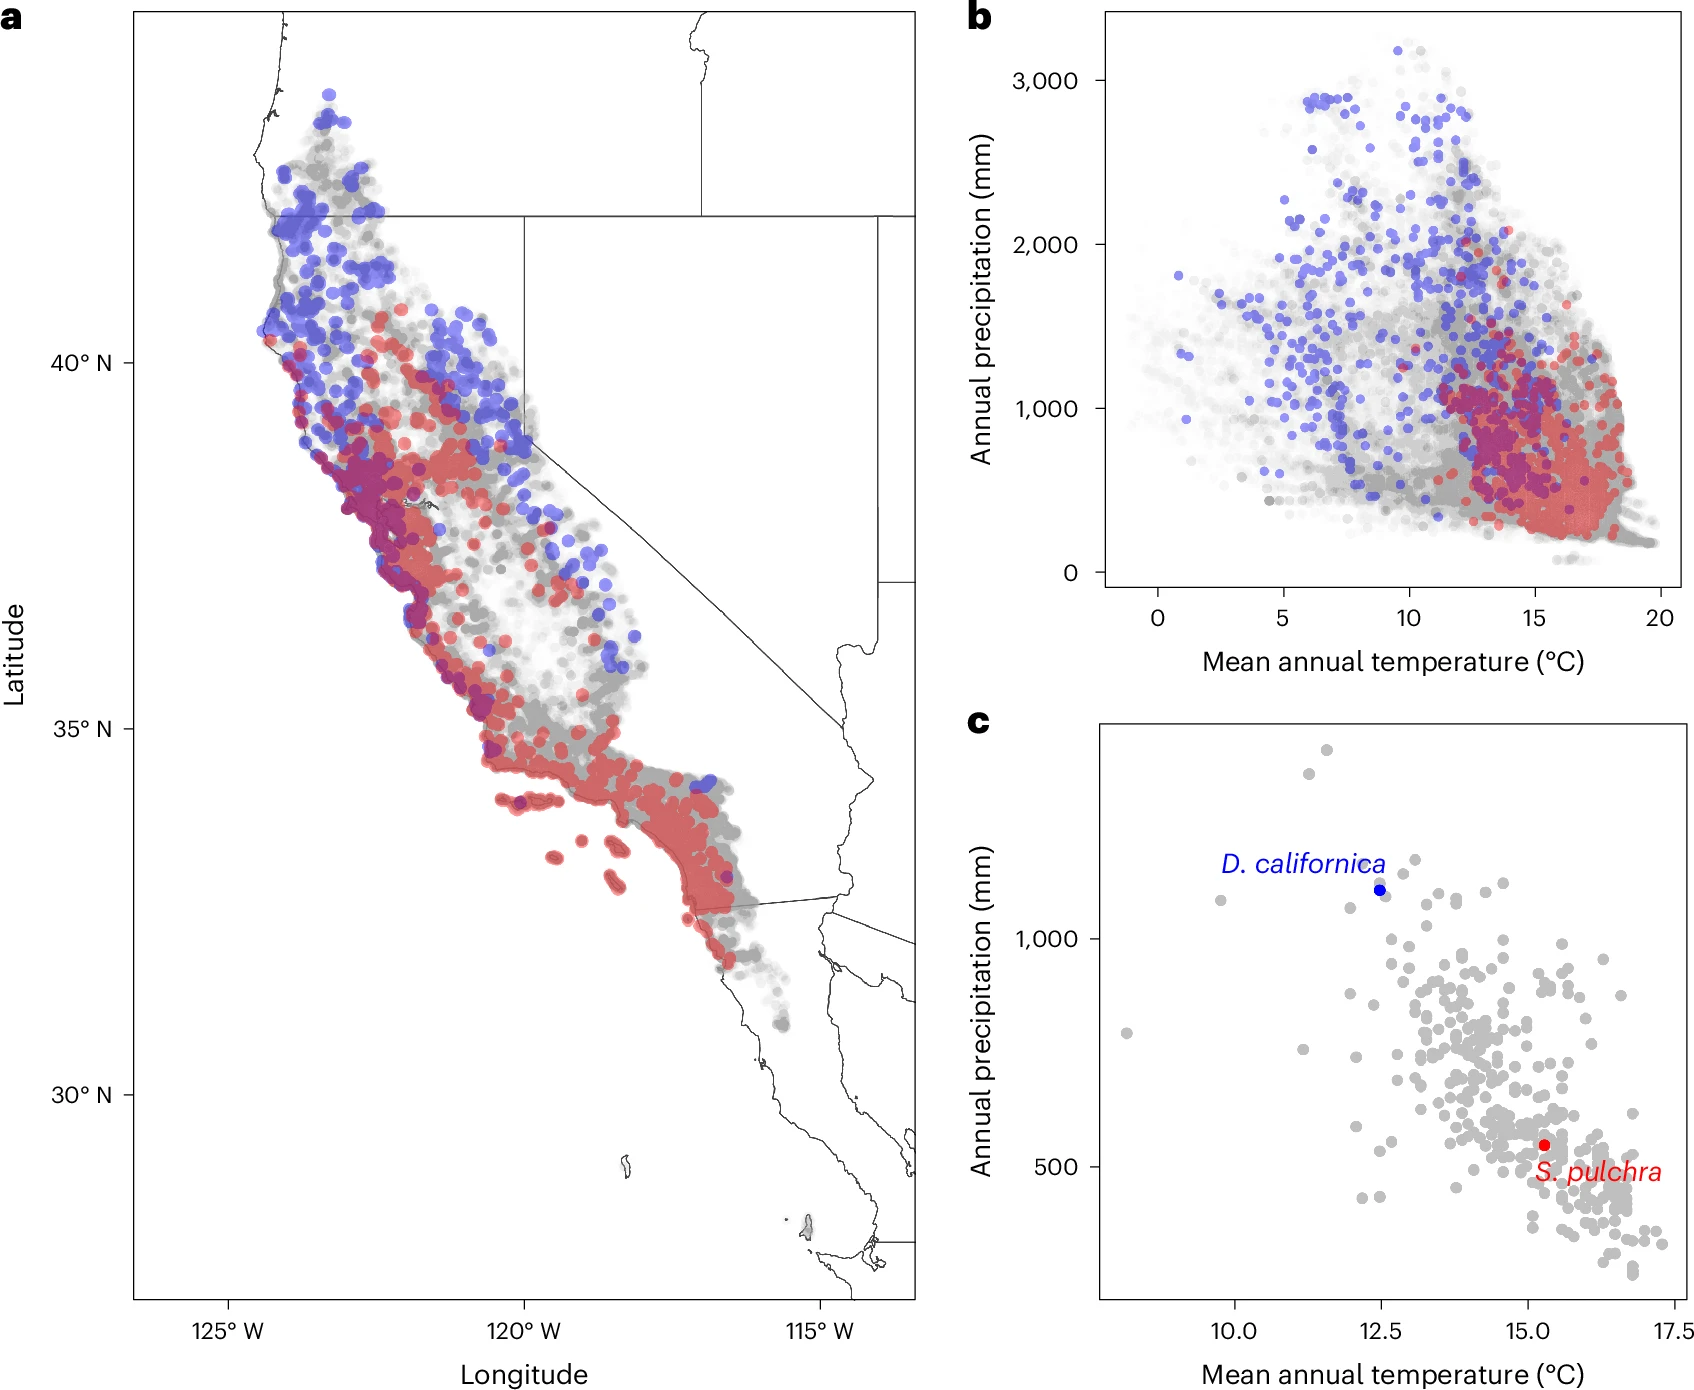
\includegraphics[width=0.9\linewidth]{../figures/grassland.png}
  \caption{\textbf{Grassland species occur along geographic and climatic gradients to estimate niches.}. a, Occurrence of grassland species in the CFP, retrieved from the GBIF data (grey points), highlighting two example species, \textit{D. californica} in the north (blue points) and \textit{S. pulchra} in the south (red points). b, Species occurrence in climate space of mean annual temperature and annual precipitation, retrieved from the CHELSA data (grey), highlighting the same two example species, \textit{D. californica} under cool and wet climates (blue) and \textit{S. pulchra} under warm and dry climates (red). c, Estimated climatic niche centroids from the medians of temperature and precipitation for each species (grey), highlighting the two species (blue and red).}
  \label{fig:grassland}
\end{figure}


\section{Discussion}
Placeholder: interpret how climate niche differentiation and interaction parameter space jointly explain coexistence outcomes, and outline implications under climate change.

\end{document}
